\documentclass[12pt,a4paper,bibliography=totocnumbered,listof=totocnumbered]{scrartcl}
\usepackage[ngerman]{babel}
\usepackage[utf8]{inputenc}
\usepackage{amsmath}
\usepackage{amsfonts}
\usepackage{amssymb}
\usepackage{graphicx}
\usepackage{fancyhdr}
\usepackage{tabularx}
\usepackage{geometry}
\usepackage{setspace}
\usepackage[right]{eurosym}
\usepackage[printonlyused]{acronym}
\usepackage{subfig}
\usepackage{floatflt}
\usepackage[usenames,dvipsnames]{color}
\usepackage{colortbl}
\usepackage{paralist}
\usepackage{array}
\usepackage{titlesec}
\usepackage{parskip}
\usepackage[right]{eurosym}
\usepackage[subfigure,titles]{tocloft}
\usepackage[pdfpagelabels=true]{hyperref}
\usepackage[rgb]{xcolor}
\usepackage[obeyFinal, colorinlistoftodos, backgroundcolor=yellow, 
linecolor=yellow, textsize=tiny, textwidth=43]{todonotes}
\usepackage{letltxmacro}
\usepackage[autostyle, german=quotes]{csquotes}
\MakeOuterQuote{"}
\usepackage{biblatex}
\usepackage{enumitem}
\usepackage{etoolbox}
\usepackage{xparse}
\usepackage{import}
\usepackage[pagewise, right]{lineno}
\usepackage{ifdraft}
\usepackage{multirow}
\usepackage{placeins}
\usepackage{longtable}

\usepackage{listings}
\lstset{basicstyle=\footnotesize, captionpos=b, breaklines=true, showstringspaces=false, tabsize=2, frame=lines, numbers=left, numberstyle=\tiny, xleftmargin=2em, framexleftmargin=2em}
\makeatletter
\def\l@lstlisting#1#2{\@dottedtocline{1}{0em}{1em}{\hspace{1,5em} Lst. #1}{#2}}
\makeatother

\geometry{a4paper, top=27mm, left=30mm, right=20mm, bottom=35mm, headsep=10mm, footskip=12mm}

\hypersetup{unicode=false, pdftoolbar=true, pdfmenubar=true, pdffitwindow=false, pdfstartview={FitH},
	pdftitle={Bachelorarbeit},
	pdfauthor={Rene Zarwel},
	pdfsubject={Microservices und technologische Heterogenität},
	pdfcreator={\LaTeX\ with package \flqq hyperref\frqq},
	pdfproducer={pdfTeX \the\pdftexversion.\pdftexrevision},
	pdfkeywords={Bachelorarbeit},
	pdfnewwindow=true,
	colorlinks=true,linkcolor=black,citecolor=black,filecolor=magenta,urlcolor=black}
\pdfinfo{/CreationDate (D:20110620133321)}

\definecolor{red}{rgb}{0.6,0,0} % for strings
\definecolor{green}{rgb}{0.25,0.5,0.35} % comments
\definecolor{purple}{rgb}{0.5,0,0.35} % keywords
\definecolor{docblue}{rgb}{0.25,0.35,0.75} % javadoc
%-------Listings Definitions------
\lstset{
	basicstyle=\footnotesize,
	keywordstyle=\color{purple}\bfseries,
	stringstyle=\color{red},
	commentstyle=\color{green},
	morecomment=[s][\color{docblue}]{/**}{*/},
	numbers=left,
	numberstyle=\tiny\color{black},
	stepnumber=2,
	tabsize=4,
	showspaces=false,
	showstringspaces=false
	captionpos=b, 
	breaklines=true, 
	frame=lines, 
	numberstyle=\tiny, 
	xleftmargin=2em, 
	framexleftmargin=2em
}
\lstdefinelanguage{Golang}
{morekeywords=[1]{package,import,func,type,struct,return,defer,panic,%
		recover,select,var,const,iota,},%
	morekeywords=[2]{string,uint,uint8,uint16,uint32,uint64,int,int8,int16,%
		int32,int64,bool,float32,float64,complex64,complex128,byte,rune,uintptr,%
		error,interface},%
	morekeywords=[3]{map,slice,make,new,nil,len,cap,copy,close,true,false,%
		delete,append,real,imag,complex,chan,},%
	morekeywords=[4]{for,break,continue,range,goto,switch,case,fallthrough,if,%
		else,default,},%
	morekeywords=[5]{Println,Printf,Error,},%
	sensitive=true,%
	morecomment=[l]{//},%
	morecomment=[s]{/*}{*/},%
	morestring=[b]',%
	morestring=[b]",%
	morestring=[s]{`}{`},%
}
%------------------------------

\numberwithin{figure}{section} %Numbering of figs include section
\numberwithin{table}{section} %Numbering of tables include section

\setlist[description]{labelindent=1cm}
\setlist[itemize]{labelindent=1cm}
\setlist[enumerate]{labelindent=1cm}

\newcommand{\newparagraph}[1]{\paragraph{#1}~\\~\\}
\newcommand{\newsubparagraph}[1]{\subparagraph{#1}~\\}

\newcommand{\acfootnote}[1]{\acs{#1}\footnote{\acf{#1}}}

% Nice and big quote
% #1 Quote
% #2 Name of person to quote
\newcommand{\bigquote}[2]{
	\vspace*{1\baselineskip}
	\begin{center}
		\begin{minipage}{0.8\textwidth}
			\enquote{\textit{#1}}\par
			- #2
		\end{minipage}
	\end{center}
	\vspace*{1\baselineskip}
}
%-----------------

%Todo Commands
\newcounter{todocounter}

\LetLtxMacro{\todoold}{\todo}
\renewcommand{\todo}[2][]{\stepcounter{todocounter}\todoold[#1]{TODO \thetodocounter: #2}}
\newcommand{\todoInline}[1]{\todo[inline]{#1}}
\newcommand{\todoFigure}[1]{\stepcounter{todocounter}\missingfigure[figcolor=white]{TODO \thetodocounter: #1}}
% ----------------

%Cite Redefinition - Auto Space on citation + Prevent forever alone citation
\renewcommand{\multicitedelim}{\addsemicolon\space}
\LetLtxMacro{\citeold}{\cite}
\renewcommand{\cite}[2][]{~\citeold[#1]{#2}}
\LetLtxMacro{\citesold}{\cites}
\DeclareDocumentCommand{\cites}{o m o m}{
	\IfNoValueTF{#1}{
		\IfNoValueTF{#3}{
			~\citesold{#2}{#4}
		}{
			~\citesold{#2}[#3]{#4}
		}
	}{
		\IfNoValueTF{#3}{
			~\citesold[#1]{#2}{#4}
		}{
			~\citesold[#1]{#2}[#3]{#4}
		}
	}
}
%----------------------

%Image Command - Optional Image otherwise TODO
% #1 IMAGE File - optional (TODO if not present)
% #2 Image options - optional
% #3 LabelName
% #4 TOC Text
% #5 Captiontext
\DeclareDocumentCommand{\image}{ o O{width=\linewidth} m m m}{
	\begin{minipage}{\linewidth}
		\vspace*{0.5cm}
		\centering
		\IfNoValueTF{#1}{
			\todoFigure{#4}
		}{
			\includegraphics[#2]{Bilder/#1}
		}	
		\captionof{figure}[#4]{#5}
		\label{#3}
		\vspace*{0.5cm}
\end{minipage}
}
%-------------

\bibliography{bibo}

\begin{document}

\titlespacing{\section}{0pt}{12pt plus 4pt minus 2pt}{-6pt plus 2pt minus 2pt}

% Kopf- und Fusszeile
\renewcommand{\sectionmark}[1]{\markright{#1}}
\renewcommand{\leftmark}{\rightmark}
\pagestyle{fancy}
\lhead{}
\chead{}
\rhead{\thesection\space\contentsname}
\lfoot{Microservices und technologische Heterogenität}
\cfoot{}
\rfoot{\ \linebreak Seite \thepage}
\renewcommand{\headrulewidth}{0.4pt}
\renewcommand{\footrulewidth}{0.4pt}

% Vorspann
\renewcommand{\thesection}{\Roman{section}}
\renewcommand{\theHsection}{\Roman{section}}
\pagenumbering{Roman}

% ----------------------------------------------------------------------------------------------------------
% Titelseite
% ----------------------------------------------------------------------------------------------------------
\thispagestyle{empty}
\begin{center}
	
\includegraphics[scale=0.5]{Bilder/Hochschule_Muenchen_Logo.png}\\
	\vspace*{2cm}
	\Large
	\textbf{Fakultät für Informatik und Mathematik 07}\\
	\vspace*{2cm}
	\Huge
	\textbf{Bachelorarbeit}\\
	\vspace*{0.5cm}
	\large
	über das Thema\\
	\vspace*{1cm}
	\textbf{Microservices und technologische Heterogenität}\\
	Entwicklung einer sprachunabhängigen Microservice Framework Evaluationsmethode\\
	\vspace*{2cm}
	
	\vfill
	\normalsize
	\newcolumntype{x}[1]{>{\raggedleft\arraybackslash\hspace{0pt}}p{#1}}
	\begin{tabular}{x{6cm}p{7.5cm}}
		\rule{0mm}{5ex}\textbf{Autor:} & René Zarwel\newline zarwel@hm.edu \\ 
		\rule{0mm}{5ex}\textbf{Prüfer:} & Prof. Dr. Hammerschall \\ 
		\rule{0mm}{5ex}\textbf{Abgabedatum:} & 13.03.2017\\ 
	\end{tabular} 
\end{center}
\pagebreak

% ----------------------------------------------------------------------------------------------------------
% Abstract
% ----------------------------------------------------------------------------------------------------------
\setcounter{page}{1}
\onehalfspacing
\titlespacing{\section}{0pt}{12pt plus 4pt minus 2pt}{2pt plus 2pt minus 2pt}
\rhead{KURZFASSUNG}
\section{Kurzfassung}
Insert Abstract Here

\vspace{-1,2em}
\titlespacing{\section}{0pt}{12pt plus 4pt minus 2pt}{-6pt plus 2pt minus 2pt}
\section*{Abstract}
Insert Abstract Here
\pagebreak

% ----------------------------------------------------------------------------------------------------------
% Verzeichnisse
% ----------------------------------------------------------------------------------------------------------
% TODO Typ vor Nummer
\renewcommand{\cfttabpresnum}{Tab. }
\renewcommand{\cftfigpresnum}{Abb. }
\settowidth{\cfttabnumwidth}{Abb. 10\quad}
\settowidth{\cftfignumwidth}{Abb. 10\quad}

\titlespacing{\section}{0pt}{12pt plus 4pt minus 2pt}{2pt plus 2pt minus 2pt}
\singlespacing
\rhead{INHALTSVERZEICHNIS}
\renewcommand{\contentsname}{II Inhaltsverzeichnis}
\phantomsection
\addcontentsline{toc}{section}{\texorpdfstring{II \hspace{0.35em}Inhaltsverzeichnis}{Inhaltsverzeichnis}}
\addtocounter{section}{1}
\tableofcontents
\pagebreak
\rhead{VERZEICHNISSE}
\listoffigures
\pagebreak
\listoftables
%\pagebreak
\renewcommand{\lstlistlistingname}{Listing-Verzeichnis}
{\labelsep2cm\lstlistoflistings}
\pagebreak
% ----------------------------------------------------------------------------------------------------------
% Abkürzungen
% ----------------------------------------------------------------------------------------------------------
\section{Abkürzungsverzeichnis}
\begin{acronym}[ATAM] % längste Abkürzung steht in eckigen Klammern
	\setlength{\itemsep}{-\parsep} % geringerer Zeilenabstand
	\acro{SEI}{Software Engineering Institute}
	\acro{SAAM}{Software Architecture Analysis Method}
	\acro{ATAM}{Architecture Tradeoff Analysis Method}
	\acro{SAEM}{Software Architecture Evaluation Model}
	\acro{GQM}{Goal Question Metrik}
	\acro{QUT}{Quality Utility Tree}
	\acro{MFEM}{Microservice Framework Evaluation Method}
	\acro{HATEOAS}{Hypermedia As The Engine Of Application State}
	\acro{REST}{Representational State Transfer}
	\acro{XML}{Extensible Markup Language}
	\acro{JSON}{JavaScript Object Notation}
	\acro{CW}{Cognitive Walkthrough}
	\acro{JWT}{JSON Web Token}
	\acro{API}{Programmierschnittstelle}
	\acro{HATEOAS}{Hypermedia As The Engine Of Application State}
	\acro{JPA}{Java Persistence API}
	\acro{LOC}{Lines of Code}
\end{acronym}
\newpage

% ----------------------------------------------------------------------------------------------------------
% Inhalt
% ----------------------------------------------------------------------------------------------------------
% Abstände Überschrift
\titlespacing{\section}{0pt}{12pt plus 4pt minus 2pt}{-6pt plus 2pt minus 2pt}
\titlespacing{\subsection}{0pt}{12pt plus 4pt minus 2pt}{-6pt plus 2pt minus 2pt}
\titlespacing{\subsubsection}{0pt}{12pt plus 4pt minus 2pt}{-6pt plus 2pt minus 2pt}

% Kopfzeile
\renewcommand{\sectionmark}[1]{\markright{#1}}
\renewcommand{\subsectionmark}[1]{}
\renewcommand{\subsubsectionmark}[1]{}
\lhead{Kapitel \thesection}
\rhead{\rightmark}

\onehalfspacing
\renewcommand{\thesection}{\arabic{section}}
\renewcommand{\theHsection}{\arabic{section}}
\setcounter{section}{0}
\pagenumbering{arabic}
\setcounter{page}{1}

%
\ifoptionfinal{}{\linenumbers}
 ----------------------------------------------------------------------------------------------------------
% Einleitung und Motivation
% ----------------------------------------------------------------------------------------------------------
\subimport{Einleitung/}{Einleitung}
\pagebreak
% ----------------------------------------------------------------------------------------------------------
% Microservices
% ----------------------------------------------------------------------------------------------------------
\subimport{Grundlagen/}{Grundlagen}
\pagebreak

% ----------------------------------------------------------------------------------------------------------
% Konzeption Methode
% ----------------------------------------------------------------------------------------------------------
\subimport{Konzeption/}{Konzeption}

\pagebreak

% ----------------------------------------------------------------------------------------------------------
% Evaluation an Beispielen
% ----------------------------------------------------------------------------------------------------------
\subimport{Evaluation/}{Evaluation}

\pagebreak

% ----------------------------------------------------------------------------------------------------------
% Zusammenfassung und Ausblick
% ----------------------------------------------------------------------------------------------------------
\subimport{Zusammenfassung/}{Zusammenfassung}

\pagebreak
\nolinenumbers
% ----------------------------------------------------------------------------------------------------------
% Literatur
% ----------------------------------------------------------------------------------------------------------
\renewcommand\refname{Quellenverzeichnis}

\printbibliography
\pagebreak

% ----------------------------------------------------------------------------------------------------------
% Todos
% ----------------------------------------------------------------------------------------------------------
\todototoc
\listoftodos
\pagebreak
% ----------------------------------------------------------------------------------------------------------
% Selbstständigkeitserklärung
% ----------------------------------------------------------------------------------------------------------
\begin{appendix}
\pagenumbering{Roman}
\setcounter{page}{1}

\thispagestyle{empty}
\section*{Selbstständigkeitserklärung}
\phantomsection
\addcontentsline{toc}{section}{Selbstständigkeitserklärung}
\addtocontents{toc}{\vspace{-0.5em}}

\vspace{2cm}
\begin{table}[!h]
	\centering
	\begin{tabular}{p{0.5\linewidth}p{0.5\linewidth}}
		\textbf{Zarwel, René} & \textbf{München, 13.03.2017} \\ 
		(Familienname, Vorname) & (Ort, Datum)\\
		\\ \\
		\textbf{21.10.1987} & \textbf{Informatik - 7B / WS - 2013} \\ 
		(Geburtsdatum) & (Studiengruppe / WS/SS)\\
	\end{tabular} 
\end{table}
\vspace{2cm}

\begin{center}
	\Large
	\textbf{Erklärung}
\end{center}

\vspace{1cm}
Hiermit erkläre ich, dass ich die Bachelorarbeit selbständig verfasst, noch nicht anderweitig für Prüfungszwecke vorgelegt, keine anderen als die angegebenen Quellen oder Hilfsmittel benutzt sowie wörtliche und sinngemäße Zitate als solche gekennzeichnet habe.\\[4ex]

München, den 13.03.2017\\[6ex]
\flushleft
\newlength\us
\settowidth{\us}{-René~Zarwel-}
\begin{tabular}{p{\us}}\hline
	\centering\footnotesize René~Zarwel
\end{tabular}
\pagebreak
% ----------------------------------------------------------------------------------------------------------
% Anhang
% ----------------------------------------------------------------------------------------------------------
\lhead{Anhang \thesection}
\section*{Anhang}
\phantomsection
\addcontentsline{toc}{section}{Anhang}
\addtocontents{toc}{\vspace{-0.5em}}
\section{\acs*{MFEM} - Vollständiger Quality Utility Tree der Basisanforderungen}
	\begin{minipage}{\linewidth}
	\centering
	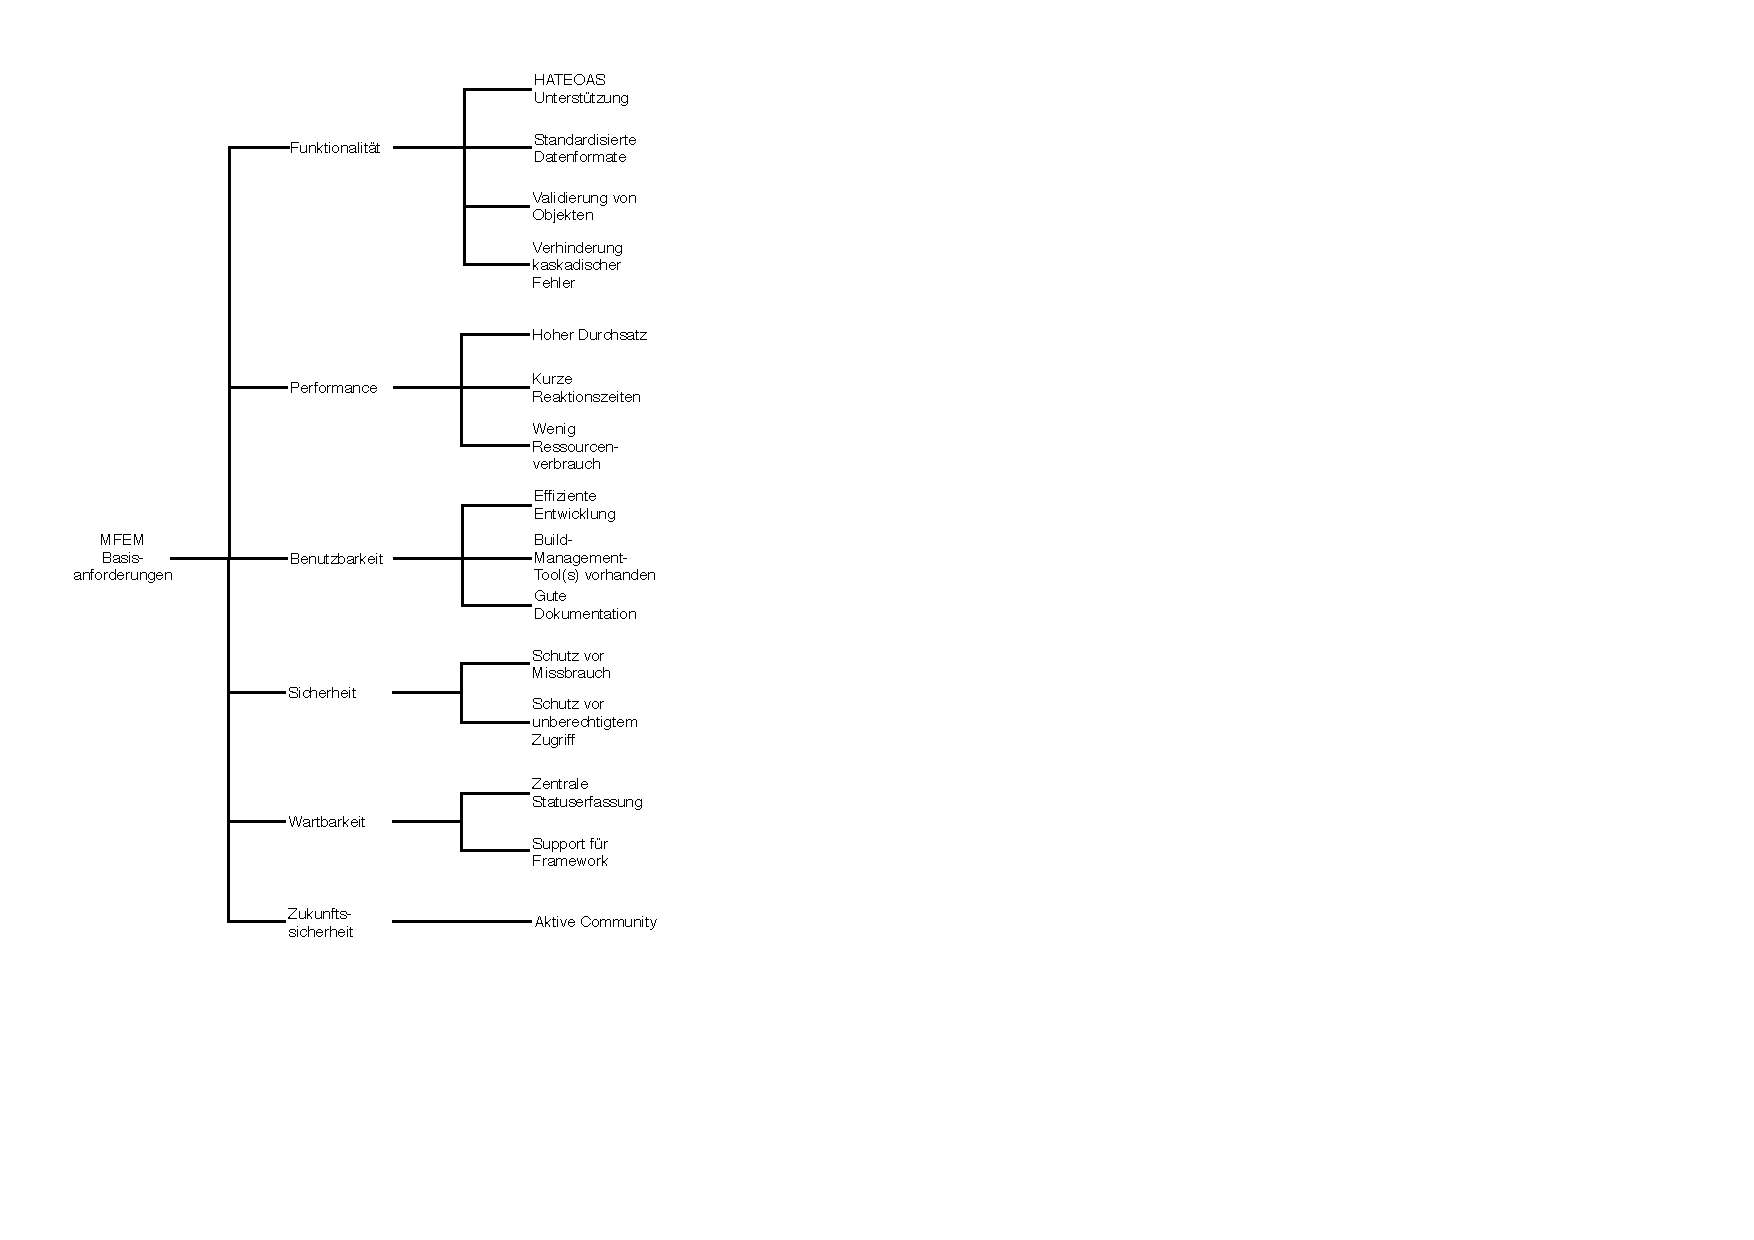
\includegraphics[width=0.8\linewidth]{Bilder/Basisanforderungen-QUT.pdf}	
	\end{minipage}
\pagebreak

\end{appendix}
\end{document}
